\documentclass[tikz,border=12pt]{standalone}
\usepackage[T1]{fontenc}
\usepackage{lmodern,amsmath}
\usetikzlibrary{arrows.meta}
\definecolor{ink}{HTML}{183444}
\definecolor{blue}{HTML}{1B6780}
\definecolor{amber}{HTML}{AD601A}
\begin{document}
\hyphenpenalty=10000\exhyphenpenalty=10000
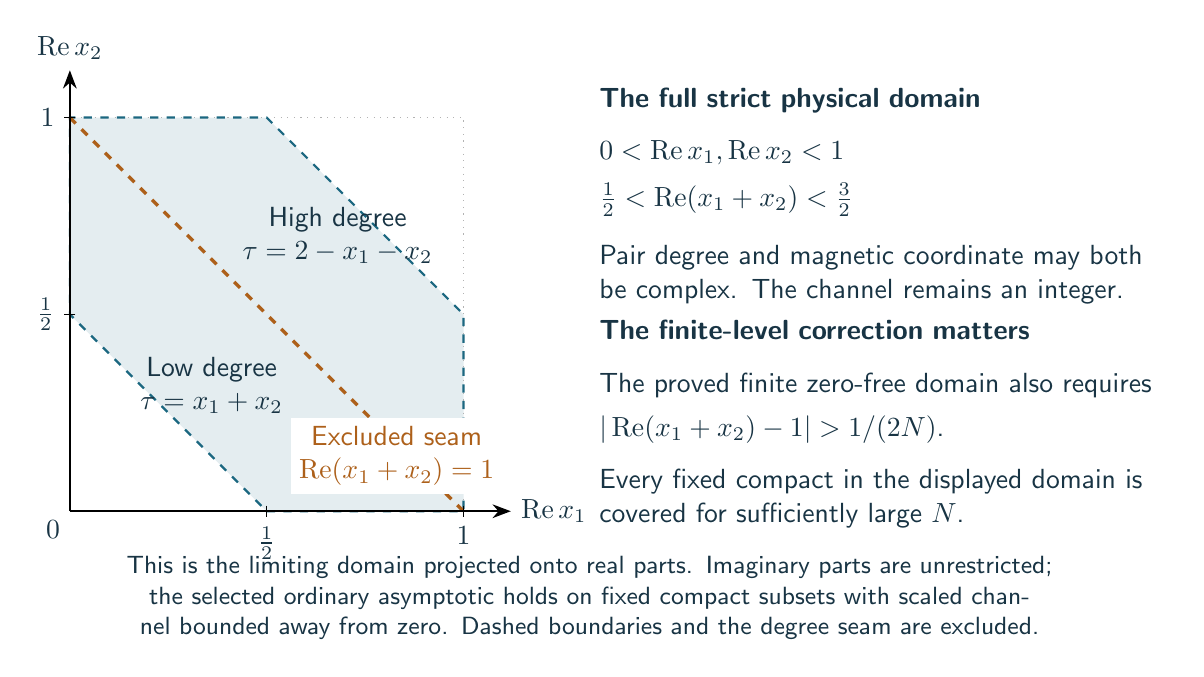
\begin{tikzpicture}[font=\sffamily,text=ink,>=Stealth]
 \fill[blue!12] (2.5,0)--(5,0)--(5,2.5)--(2.5,5)--(0,5)--(0,2.5)--cycle;
 \draw[gray!60,dotted] (0,0) rectangle (5,5);
 \draw[blue,thick,dashed] (2.5,0)--(5,0)--(5,2.5)--(2.5,5)--(0,5)--(0,2.5)--cycle;
 \draw[amber,very thick,dashed] (0,5)--(5,0);
 \draw[->,thick] (0,0)--(5.6,0) node[right] {$\operatorname{Re}x_1$};
 \draw[->,thick] (0,0)--(0,5.6) node[above] {$\operatorname{Re}x_2$};
 \foreach \v/\lab in {2.5/{\tfrac12},5/{1}} {
   \draw (\v,.07)--(\v,-.07) node[below] {$\lab$};
   \draw (.07,\v)--(-.07,\v) node[left] {$\lab$};
 }
 \node[below left] at (0,0) {$0$};
 \node[align=center] at (1.8,1.6) {Low degree\\$\tau=x_1+x_2$};
 \node[align=center] at (3.4,3.5) {High degree\\$\tau=2-x_1-x_2$};
 \node[amber,align=center,fill=white,inner sep=3pt] at (4.15,.7) {Excluded seam\\$\operatorname{Re}(x_1+x_2)=1$};
 \node[anchor=north west,align=left,text width=7.2cm] at (6.6,5.5) {
   \textbf{The full strict physical domain}\\[7pt]
   $0<\operatorname{Re}x_1,\operatorname{Re}x_2<1$\\[5pt]
   $\tfrac12<\operatorname{Re}(x_1+x_2)<\tfrac32$\\[9pt]
   Pair degree and magnetic coordinate may both be complex.
   The channel remains an integer.};
 \node[anchor=north west,align=left,text width=7.2cm] at (6.6,2.55) {
   \textbf{The finite-level correction matters}\\[7pt]
   The proved finite zero-free domain also requires\\[4pt]
   $|\operatorname{Re}(x_1+x_2)-1|>1/(2N)$.\\[7pt]
   Every fixed compact in the displayed domain is covered for
   sufficiently large $N$.};
 \node[align=center,text width=13cm,font=\sffamily\small] at (6.6,-1.1) {
   This is the limiting domain projected onto real parts. Imaginary parts are unrestricted;
   the selected ordinary asymptotic holds on fixed compact subsets with scaled channel bounded away from zero.
   Dashed boundaries and the degree seam are excluded.};
\end{tikzpicture}
\end{document}
